% Chapter 3

\chapter{Introduction to the Player Study}

\label{chapter:player-study-introduction}
\lhead{Chapter \ref{chapter:player-study-introduction}. \emph{Player Study - Introduction}}

To find answers to the research questions defined in Chapter \ref{chapter:research-questions}, a survey was constructed to be distributed among Pokémon GO players. The final version of the survey can be found in Appendix \ref{appendix:survey}. The data from the survey have been analyzed in this and the three following chapters, with interviews conducted in conjunction with a follow-up survey providing additional depth in some areas. It should be noted that most percentages have been rounded to the nearest integer, causing the sum of all percentages in some tables to exceed or fall short of 100 \%.

% Section 1 - Mapping to research questions
\section{Survey Construction}

This section will provide a mapping between the questions of the survey and the research questions each of them aim to answer. It should be noted that in addition to the listed questions, the survey included other questions intending to get further information that could either be used to provide background on the respondents or possibly reveal perspectives not previously considered. It also included a comment section at the end where respondents could provide any additional info they did not find a proper place for, and these comments have also been used to evaluate the research questions.

The first research goal, examining the success factors of Pokémon GO as seen in Section \ref{rg1}, was decomposed into five research questions, \ref{RQ1.1} through \ref{RQ1.5}. Table \ref{tbl:rg1-survey-questions} shows the survey questions relevant for this research goal and the research questions each of them help answering.

\begin{table}[h]
	\caption{\emph{What are the main factors that made Pokémon GO successful?} Survey Questions}
	\centering
	\label{tbl:rg1-survey-questions}
	\begin{tabularx}{\textwidth}{|X|l|}
		\hline
		\textbf{Survey question} & \textbf{Research questions}\\
		\hline\hline
		
		Which of the following factors influenced your decision to start playing Pokémon Go? & \ref{RQ1.1}\\
		\hline
		
		Which of the following game features do you use? & \ref{RQ1.2}\\
		\hline
		
		If you have previously played any location-based or augmented reality games, what did you like about them and what did you not like about them? How does Pokémon Go compare on these points? & \ref{RQ1.3}\\
		\hline
		
		If you have previously played any other casual mobile games, what did you like about them and what did you not like about them? How does Pokémon Go compare on these points? & \ref{RQ1.3}\\
		\hline
		
		If you have previously played any other Pokémon games, what did you like about them and what did you not like about them? How does Pokémon Go compare on these points? & \ref{RQ1.4}\\
		\hline
		
		If you are no longer playing, when and why did you stop? If you are still playing, but have greatly reduced the amount you play, when and why did this happen? & \ref{RQ1.5}\\
		\hline
	\end{tabularx}
\end{table}

The second research goal, evaluating the physical health effect of playing Pokémon GO as seen in section \ref{rg2} was decomposed into six research questions, \ref{rq-physical-activity-amount} through \ref{rq-physical-risks}. Table \ref{tbl:rg2-survey-questions} shows the survey questions relevant for this research goal and the research questions each of them help answering.

\begin{table}[h]
	\caption{\emph{What are the effects on physical health from playing Pokémon GO, and how much effort does it take to achieve this effect?} Survey Questions}
	\centering
	\label{tbl:rg2-survey-questions}
	\begin{tabularx}{\textwidth}{|X|l|}
		\hline
		\textbf{Survey question} & \textbf{Research questions}\\
		\hline\hline
		
		In an average week, how much time did you spend on physical activities (e.g. walking, running or biking) before you started playing Pokémon Go? & \ref{rq-physical-activity-amount}, \ref{rq-physical-high-low-comparison}\\
		\hline
		
		In an average week, how much time do you spend on physical activities since you started playing Pokémon Go? & \ref{rq-physical-activity-amount}, \ref{rq-physical-high-low-comparison}\\
		\hline
		
		If you spend more time on physical activities after you started playing Pokémon Go than before, what are the sources of this activity? & \ref{rq-physical-game-activities}\\
		\hline
		
		Have you lost weight or in other ways feel more healthy than before you started playing Pokémon Go? & \ref{rq-physical-weight-loss}\\
		\hline
		
		Have you skipped out on less healthy activities (e.g. going out to drink) that you otherwise would have engaged in due to playing Pokémon Go instead? If so, please specify. & \ref{rq-physical-unhealthy-habits}\\
		\hline
		
		Have you trespassed or otherwise gone into areas you shouldn’t be because you were playing Pokémon Go? & \ref{rq-physical-risks}\\
		\hline
		
		Have you put yourself or others in dangerous situations because you were playing Pokémon Go? & \ref{rq-physical-risks}\\
		\hline
		
		Have you gotten into any accidents because either you or another involved party was playing Pokémon Go? & \ref{rq-physical-risks}\\
		\hline
		
		If you have put yourself or others in dangerous situations, or gotten into accidents, because of Pokémon Go, could you elaborate? & \ref{rq-physical-risks}\\
		\hline
		
		Have you neglected other areas of your life because you were playing Pokémon Go? & \ref{rq-physical-risks}\\
		\hline
	\end{tabularx}
\end{table}

The third research goal, evaluating the mental health effect of playing Pokémon GO as seen in section \ref{rg2} was decomposed into four research questions, \ref{rq-mental-social-activity-amount} through \ref{rq-mental-illnesses}. Table \ref{tbl:rg3-survey-questions} shows the survey questions relevant for this research goal and the research questions each of them help answering.

\begin{table}[h]
	\caption{\emph{What are the effects on mental health from playing Pokémon GO?} Survey Questions}
	\centering
	\label{tbl:rg3-survey-questions}
	\begin{tabularx}{\textwidth}{|X|l|}
		\hline
		\textbf{Survey question} & \textbf{Research questions}\\
		\hline\hline
		
		In an average week, during your spare time, how much time did you spend socializing with other people (in person, outside your home) before you started playing Pokémon Go? & \ref{rq-mental-social-activity-amount}\\
		\hline
		
		In an average week, during your spare time, how much time do you spend socializing with other people (in person, outside your home) since you started playing Pokémon Go? & \ref{rq-mental-social-activity-amount}\\
		\hline
		
		If you have increased the amount of time you spend socializing with people since you started playing Pokémon Go than before, what are the causes of this increase? & \ref{rq-mental-game-activities}\\
		\hline
		
		Have you talked to someone in person because of Pokémon Go that you otherwise would not have talked to? & \ref{rq-mental-relationships}, \ref{rq-mental-illnesses}\\
		\hline
		
		Have you made new friends through playing the game? & \ref{rq-mental-relationships}\\
		\hline
		
		Has playing Pokémon Go improved any of your existing relationships? & \ref{rq-mental-relationships}\\
		\hline
		
		Do you suffer from any mental illnesses? & \ref{rq-mental-illnesses}\\
		\hline
		
		If you suffer from a mental illness, do you feel that playing Pokémon Go has had a positive effect on your mental health? If yes, feel free to elaborate on how it has helped you & \ref{rq-mental-illnesses}\\
		\hline
	\end{tabularx}
\end{table}
\clearpage

% Section 2 - Survey distribution
\section{Survey Distribution}
\label{sec:survey-distribution}

The survey was distributed in a Norwegian and an English version, and in multiple phases. After the first phase, some questions were adjusted, and a missing question regarding weight loss and perceived improvement on physical health was added.

The first phase of distribution took place at a large Pokémon Go event in \emph{Frognerparken} in Oslo, Norway, a large sculpture park and popular destination for Pokémon Go players due to the high density of Pokéstops and spawns. The survey was available online via an easily accessible custom URL from a known link shortener, leading to the Norwegian version. Single players and groups of players were approached over the span of about two hours, given a short introduction to the project and asked whether they would be willing to respond to the survey. Given a positive response, they were handed a note with the URL. Extra effort was made to reach out to players in the following categories: Young children (15 or below), parents playing with children, and players above 40. This was done in an attempt to reach the broad spectrum of ages participating, even though the bulk of players are between the ages of 20 and 35. Unfortunately, this only resulted in a very small portion of the responses collected, with 74 people following the link, and not all of them filling out the survey.

In the second phase, the survey was distributed on \emph{Facebook}. A post explaining the project and an encouragement to respond despite the length of the survey, along with links to both versions, was shared in each of the four largest Norwegian Pokémon Go groups (\emph{Pokémon GO: Norway}, \emph{Pokemon Go Norge}, \emph{Pokémon GO - Oslo \& Akershus} and \emph{Pokémon GO Trondheim}), as well as personally. It was then re-shared by several people to their local Pokémon GO groups or their personal friends and followers. These groups consisted of between 4 000 and 16 000 members, and despite overlap between groups it is not unlikely that more than 20 000 people were able to see the posts in these groups. This is where the majority of the responses originated from, with roughly 1900 clicks on the links from Facebook, yielding between 1050 and 1200 responses.

The third phase involved sharing the survey on the popular internet forum \emph{Reddit}. Here it was shared in two \emph{subreddits}, sub-forums on the larger site with their own dedicated communities. The first subreddit was \emph{/r/PokemonGo}, the main community for people interested in the game in general. The second, \emph{/r/TheSilphRoad}, is a community devoted to research on all things related to Pokémon GO.

In addition to the three main phases of distribution, people encountered playing or talking about the game at any time were approached and asked to participate throughout all of September.

In early December, the respondents who had left contact information were contacted with a short follow-up survey, seen in Appendix \ref{appendix:follow-up}. Those who had left comments of note separating them from the other respondents were additionally asked about these points of interest. This round of follow-ups was an attempt to gather information on the longevity of the game, some clarifications of questions and comments from the original survey, and answers to some new questions. All responses to the follow-up survey were carefully read and any new points of interest were further followed up on, resulting in a few interviews.

% Section 3 - Demographics
\section{Demographics}
\label{sec:player-study-demographics}

The survey collected data on the demographics of its respondents, including the age, gender and the country in which most of their playing occurred. The recorded nation is assumed to be their country of residence in most cases. A total of 2190 responses were recorded with demographic data.

Out of everyone who responded, 1244 (slightly below 57 \%) were male and 946 were female. Figure \ref{fig:respondents-age-histogram} shows a histogram of the ages of all respondents, ranging from 5 to 67 years old, with the largest number of respondents (176) being aged 25. Respondents have also been divided into seven different age groups, show in Table \ref{tbl:survey-age-distribution}. Note that the total percentages are rounded, and rounding errors cause the total to sum up to 101 \%.

\begin{figure}[h]
	\centering
	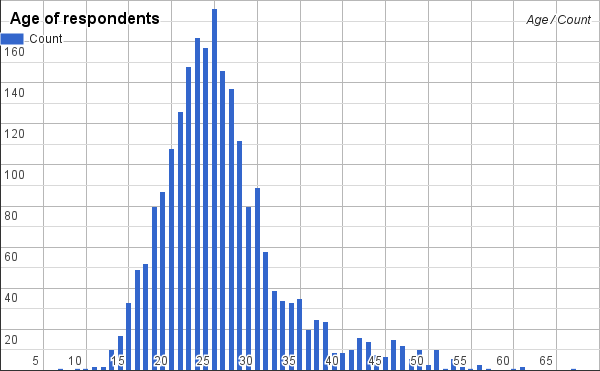
\includegraphics[width=\textwidth]{Figures/age-histogram}
	\caption{A histogram of the ages of the respondents}
	\label{fig:respondents-age-histogram}
\end{figure}

\begin{table}[h]
	\centering
	\caption{Age distribution of survey respondents}
	\label{tbl:survey-age-distribution}
	\begin{tabular}{|l||c|c|c|c|c|c|c|}
		\hline
		&\textbf{18-} & \textbf{18-21} & \textbf{22-26} & \textbf{27-32} & \textbf{33-40} & \textbf{41-50} & \textbf{50+}\\
		\hline\hline
		\textbf{Male} & 120 & 247 & 434 & 284 & 108 & 37 & 14 \\
		\hline
		\textbf{Female} & 48 & 154 & 355 & 231 & 81 & 64 & 14 \\
		\hline
		\textbf{Total} & 168 & 401 & 789 & 515 & 189 & 101 & 28 \\
					& 8\% & 18\% & 36\% & 24\% & 9\% & 5\% & 1\%\\
		\hline
	\end{tabular}
\end{table}

If we normalize the results for gender, we get the numbers in Table \ref{tbl:survey-age-distribution-normalized}. From this we can see that the game seemed to be more popular among males in the younger categories, while the older categories showed a preference towards female players. The middle categories were more even. This fits observations of players \emph{in the wild}. Groups of young boys were a common sight, but young girls were much more rare. Mothers aged 40 and above playing with children also seemed more common than fathers around that age doing the same, and walking groups consisting of women also seemed more common than male equivalents.

\begin{table}[h]
	\centering
	\caption{Age distribution of respondents normalized for gender}
	\label{tbl:survey-age-distribution-normalized}
	\begin{tabular}{|l||c|c|c|c|c|c|c|}
		\hline
		&\textbf{18-} & \textbf{18-21} & \textbf{22-26} & \textbf{27-32} & \textbf{33-40} & \textbf{41-50} & \textbf{50+}\\
		\hline\hline
		\textbf{Male} & 66\% & 55\% & 48\% & 48\% & 50\% & 31\% & 43\% \\
		\hline
		\textbf{Female} & 34\% & 45\% & 52\% & 52\% & 50\% & 69\% & 57\% \\
		\hline
	\end{tabular}
\end{table}

The results contained 1189 responses stating Norway as their main location for playing, which is more than 50 \% of all responses. Because the survey was distributed in Norwegian Facebook groups, but not in local communities for other countries, Norway has been excluded from Table \ref{tbl:demographics-continents}, which shows the distribution of players per continent for the remaining respondents.

\begin{table}[h]
	\centering
	\caption{Distribution of respondents per continent}
	\label{tbl:demographics-continents}
	\begin{tabular}{|c|c|c|c|c|c|}
		\hline
		\textbf{North America} & \textbf{South America} & \textbf{Europe} & \textbf{Asia} & \textbf{Oceania} & \textbf{Africa}\\
		\hline\hline
		649		& 25	& 230	& 36	& 51	& 1\\
		65\%	& 3\%	& 23\%	& 4\%	& 5\%	& 0\%\\\hline
	\end{tabular}
\end{table}

Of the remaining responses, The United States of America has a clear overweight with 575 responses, almost half the amount of Norwegian responses. If we also exclude these respondents, more than half of the remaining responses come from Europe, with the rest being relatively evenly divided between Oceania, Asia and South America. Countries with many responses include Canada, the British Isles (the United Kingdom and Ireland), Germany, Australia and the Netherlands. The game had just been rolled out in the first parts of Africa at the time the survey concluded, and thus we only have one respondent residing in South Africa.

The survey also asked for the main occupation of each respondent, with four categories available: employed, unemployed, higher education (e.g. university or college) and lower education (e.g. high school or middle school). The following table again shows the distribution between these categories.

\begin{table}[h]
	\centering
	\caption{Distribution of survey respondents across occupations}
	\label{tbl:survey-occupation-distribution}
	\begin{tabular}{|c|c|c|c|}
		\hline
		\textbf{Lower education} & \textbf{Higher education} & \textbf{Employed} & \textbf{Unemployed}\\
		\hline\hline
		219 & 747 & 1056 & 169\\
		10\% & 34\% & 48\% & 8\%\\
		\hline
	\end{tabular}
\end{table}

The average player level of the respondents was slightly above 23, with the vast majority being in the 21-30 range. Table \ref{tbl:survey-level-distribution} shows the number of respondents in each range of levels from 1-10 through 31-40. It also shows the average number of different Pokémon caught for each level range.

\begin{table}[h]
	\centering
	\caption{Respondents and average Pokédex count per level range}
	\label{tbl:survey-level-distribution}
	\begin{tabular}{|l||c|c|c|c|}
		\hline
		& \textbf{1-10} & \textbf{11-20} & \textbf{21-30} & \textbf{31-40}\\
		\hline\hline
		\textbf{Respondents}	& 21	& 386	& 1743	& 38\\
								& 1\%	& 18\%	& 80\%	& 2\%\\\hline
		\textbf{Avg. Pokédex count} & 37 & 71 & 108 & 139\\\hline
	\end{tabular}
\end{table}
